\chapter{Software Development}
\label{chap:software-development}

\section{Software Development Methodology}
\label{section:software-development-methodology}
For earlier stages of KU Eater development, we insisted in separating our project's components' responsibilities.
Each of the components, Backend, Frontend and Recommendation Engine are done in separated repositories, and will come together in a form of a microservices architecture.

For the methodology in doing so, we decided to do bi-weekly sprints of which we called "milestones." We hold regular meetings on every 1st and 16th on each month.
We also have impromptu meetings out of schedule as well, if we encountered problems or require affirmation from each team member.

Contacting with our advisor is also encouraged if there's any serious matter that's need to be discussed.

\section{Technology Stack}
\label{section:technology-stack}
Our technology stack has been briefly covered in section \ref{section:development-system}, the following is a figure that shows a bigger picture of KU Eater's technical implementations.
\begin{figure}[H]
    \centering
    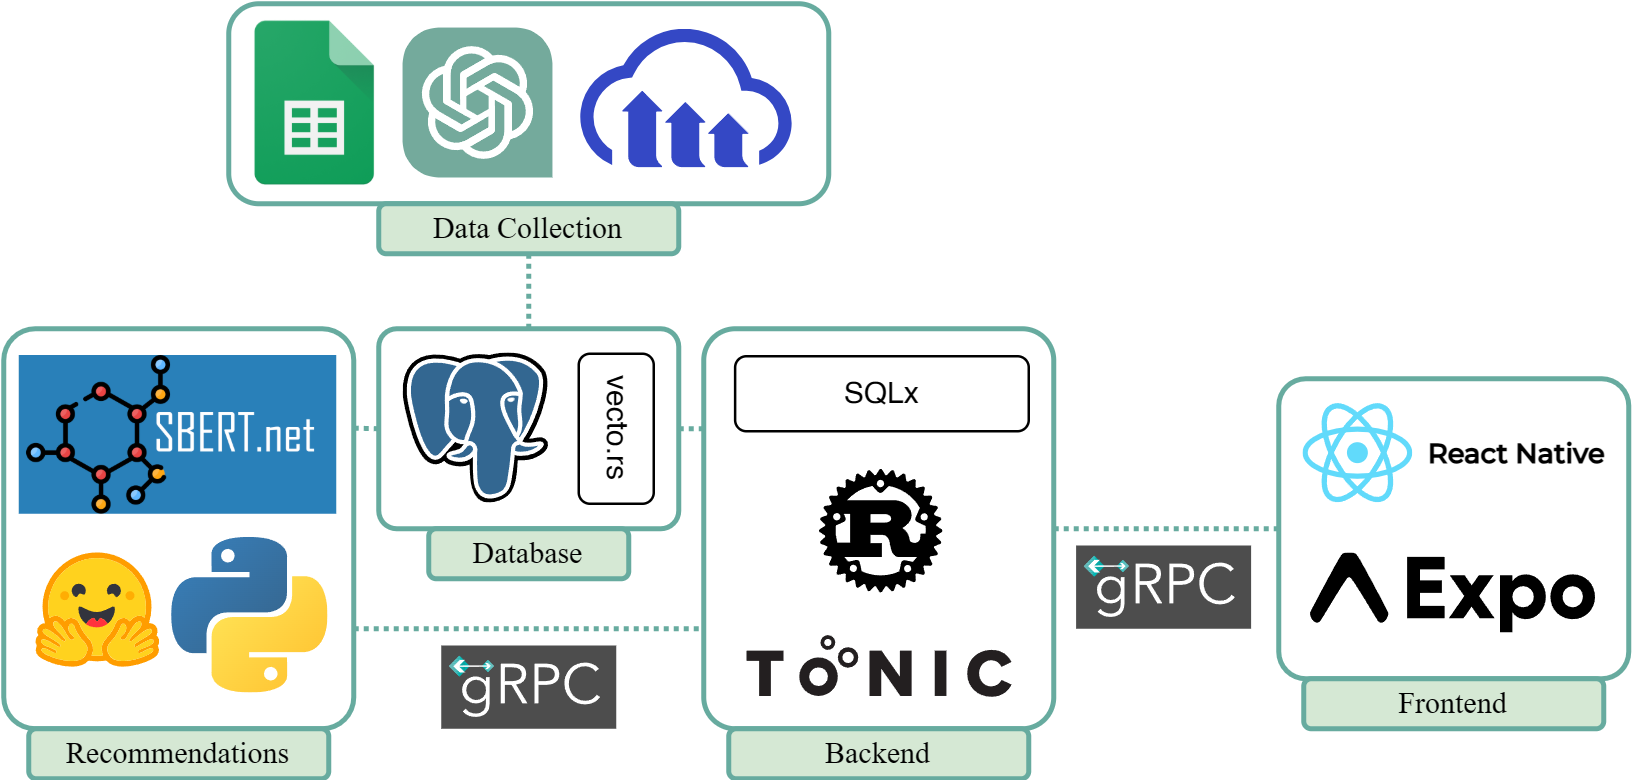
\includegraphics[width=\textwidth,height=0.3\textheight,keepaspectratio]{kueater/tech_stack.png}
    \caption{Technology Stack for KU Eater}
    \label{fig:tech-stack}
\end{figure}
From figure \ref{fig:tech-stack}, we have separate the responsibilities of technologies to five different groups: Data Collection, Database, Recommendations, Backend and Frontend.

\subsection{Data Collection}
\begin{itemize}[leftmargin=80pt]
    \item \textbf{Google Sheets:} A spreadsheet tool where we use to record interview results from stalls. Data includes stall information, list of menu items,
    prices of menu items etc. This tool is used in stages where data collection needs to be easy and fast. Moreover, since this is on cloud it can be used in later
    development stages where we require our spreadsheet to be primary data source.
    \item \textbf{OpenAI ChatGPT:} A chat tool running on large language models, it allows us to be able to infer a list of ingredients for menu items we recorded.
    The tool allows us to fill in the gaps of missing data.
\end{itemize}

\subsection{Database}
\begin{itemize}[leftmargin=80pt]
    \item \textbf{PostgreSQL:} Our choice of relational database system with plethora of features that reduce usage of complex queries
    and an extensible ecosystem.
    \item \textbf{pgvector:} An extension for PostgreSQL that allows our database to store and compare data vectors.
\end{itemize}

\subsection{Recommendations and Backend}
\begin{itemize}[leftmargin=80pt]
    \item \textbf{Rust:} A general-purpose programming language that emphasizes on type safety and performance. It has a large ecosystem of tools required for building KU Eater.
    \item \textbf{Tonic:} A gRPC server/client implementation for Rust with asynchronous support. It also has codegen tools to automatically build systems from protocol buffers.
    \item \textbf{SQLx:} A generic asynchronous SQL library for Rust.
    \item \textbf{Polars:} A dataframe library that can load from multiple data sources, including full SQL support.
    \item \textbf{Huggingface's Libraries:} We use Candle from Huggingface to create native-Rust AI models.
\end{itemize}

\subsection{Frontend}
\begin{itemize}[leftmargin=80pt]
    \item \textbf{React Native:} A web application framework that runs as native applications on mobile platforms. It allows an application to elevate
    its ability to use native components on your phone (e.g. storage, GPS)
    \item \textbf{Expo:} An extension to React Native framework with rapid prototyping support and contains extra implementations of native components.
\end{itemize}

\section{Coding Standards}
\label{section:coding-standards}
For naming conventions in any language, we try to stick to the convention which is default for each language.
For Rust implementations, it needs to conform to RFC 430 from the Rust Lang Style Guide. \cite{rustlangstyleguide}
For React Native implementations, it should respect the style guide created by Airbnb. \cite{airbnbreactstyleguide}
For Protocol Buffers, it needs to follow the style guide provided by Google. \cite{protobufstyleguide}

In communications between each components in our architecture, the communication protocol used is gRPC. It is a Remote Call Procedure framework made by Google that can be run
in any modern environment including web applications. It allows us to define our service by using Protocol Buffers language, then it can generate source code for
any programming languages to implement those services.
The advantages of using gRPC is that we will have a consistent routing pattern for our services, it is more performant than typical REST APIs
since the underlying data is transported in binary form.

\section{Progress Tracking Report}
\label{section:progress-tracking-report}
\subsection{Current Situation}
We have been working on our project and trying to follow the timeline (\ref{section:timeline}) we laid out. However, it is come to clear that
we've been working too much on proof of concept especially for backend part, the result is not to be happy with.

\begin{figure}[H]
    \centering
    \includegraphics[width=0.5\textwidth]{kueater/frontend-contribution.png}
    \caption{Frontend Contribution Graph as of 16/02/2025}
    \label{fig:frontend-contribution}
\end{figure}

\begin{figure}[H]
    \centering
    \includegraphics[width=0.5\textwidth]{kueater/backend-contribution.png}
    \caption{Backend Contribution Graph as of 16/02/2025}
    \label{fig:backend-contribution}
\end{figure}

From figure \ref{fig:frontend-contribution}, there has been significant proof of work on frontend as seen in the contribution graph.
However from figure \ref{fig:backend-contribution}, there has been a large gap before the work can actually start. This is because, the backend
is more takes more time for working and studying in a sandbox rather being developed. Extra repositories like shared protocol buffers, Docker image registries and
embedding model also require time from backend development to be allotted into them. This could be a disadvantage of microservice architecture where
we need to focus on multiple components at once.

\subsection{Extra Tools}
We used a project management tool called Linear in order to track our tasks.
\begin{figure}[H]
    \centering
    \includegraphics[width=\textwidth]{kueater/linear.png}
    \caption{Project Task Board for KU Eater}
    \label{fig:linear}
\end{figure}

\section{Committee Rebuttal (after 19/02/2025)}
\label{section:2nd-update-rebuttal}
After presenting the project's progress to committees on the 19th, February 2025, there were some issues and concerns raised by the committees.
Each sub-section is a concern that the committee raised, and within the sub-section is our approach to the issue.

\subsection*{Shouldn't the authors prioritize main features first like the Recommendation system?}
We fully agree on that statement, our management seems off and we didn't really focus on making our recommendation engine ready for the progress update.
From now on, we are going to be prioritizing building the core components like so:
\begin{itemize}[leftmargin=80pt]
    \item Recommendation engine
    \item Embedding generation agent---a service to help generate text embeddings in background to be used in other components.
    \item Search engine
    \item Backend
    \item Frontend
\end{itemize}

\subsection*{Clarify on how the Recommendation engine will work.}
This component is the heart of the entire system, and is the main feature of KU Eater. We thought that our recommendation engine should have
its own section since, it will be worked on and updated frequently. See the details of our engine at Appendix \ref{appendix:A}.